% Options for packages loaded elsewhere
\PassOptionsToPackage{unicode}{hyperref}
\PassOptionsToPackage{hyphens}{url}
\PassOptionsToPackage{dvipsnames,svgnames,x11names}{xcolor}
%
\documentclass[
  11pt,
  letterpaper,
  DIV=11,
  numbers=noendperiod]{scrreprt}

\usepackage{amsmath,amssymb}
\usepackage{iftex}
\ifPDFTeX
  \usepackage[T1]{fontenc}
  \usepackage[utf8]{inputenc}
  \usepackage{textcomp} % provide euro and other symbols
\else % if luatex or xetex
  \usepackage{unicode-math}
  \defaultfontfeatures{Scale=MatchLowercase}
  \defaultfontfeatures[\rmfamily]{Ligatures=TeX,Scale=1}
\fi
\usepackage{lmodern}
\ifPDFTeX\else  
    % xetex/luatex font selection
\fi
% Use upquote if available, for straight quotes in verbatim environments
\IfFileExists{upquote.sty}{\usepackage{upquote}}{}
\IfFileExists{microtype.sty}{% use microtype if available
  \usepackage[]{microtype}
  \UseMicrotypeSet[protrusion]{basicmath} % disable protrusion for tt fonts
}{}
\makeatletter
\@ifundefined{KOMAClassName}{% if non-KOMA class
  \IfFileExists{parskip.sty}{%
    \usepackage{parskip}
  }{% else
    \setlength{\parindent}{0pt}
    \setlength{\parskip}{6pt plus 2pt minus 1pt}}
}{% if KOMA class
  \KOMAoptions{parskip=half}}
\makeatother
\usepackage{xcolor}
\usepackage[margin=1in]{geometry}
\setlength{\emergencystretch}{3em} % prevent overfull lines
\setcounter{secnumdepth}{5}
% Make \paragraph and \subparagraph free-standing
\ifx\paragraph\undefined\else
  \let\oldparagraph\paragraph
  \renewcommand{\paragraph}[1]{\oldparagraph{#1}\mbox{}}
\fi
\ifx\subparagraph\undefined\else
  \let\oldsubparagraph\subparagraph
  \renewcommand{\subparagraph}[1]{\oldsubparagraph{#1}\mbox{}}
\fi


\providecommand{\tightlist}{%
  \setlength{\itemsep}{0pt}\setlength{\parskip}{0pt}}\usepackage{longtable,booktabs,array}
\usepackage{calc} % for calculating minipage widths
% Correct order of tables after \paragraph or \subparagraph
\usepackage{etoolbox}
\makeatletter
\patchcmd\longtable{\par}{\if@noskipsec\mbox{}\fi\par}{}{}
\makeatother
% Allow footnotes in longtable head/foot
\IfFileExists{footnotehyper.sty}{\usepackage{footnotehyper}}{\usepackage{footnote}}
\makesavenoteenv{longtable}
\usepackage{graphicx}
\makeatletter
\def\maxwidth{\ifdim\Gin@nat@width>\linewidth\linewidth\else\Gin@nat@width\fi}
\def\maxheight{\ifdim\Gin@nat@height>\textheight\textheight\else\Gin@nat@height\fi}
\makeatother
% Scale images if necessary, so that they will not overflow the page
% margins by default, and it is still possible to overwrite the defaults
% using explicit options in \includegraphics[width, height, ...]{}
\setkeys{Gin}{width=\maxwidth,height=\maxheight,keepaspectratio}
% Set default figure placement to htbp
\makeatletter
\def\fps@figure{htbp}
\makeatother

\usepackage{booktabs}
\usepackage{caption}
\usepackage{longtable}
\usepackage{colortbl}
\usepackage{array}
\KOMAoption{captions}{tableheading}
\usepackage{graphicx}
\usepackage{fontspec}
\setmainfont{Times New Roman}
\usepackage{geometry}
\pagestyle{empty}
\makeatletter
\@ifpackageloaded{bookmark}{}{\usepackage{bookmark}}
\makeatother
\makeatletter
\@ifpackageloaded{caption}{}{\usepackage{caption}}
\AtBeginDocument{%
\ifdefined\contentsname
  \renewcommand*\contentsname{Table of contents}
\else
  \newcommand\contentsname{Table of contents}
\fi
\ifdefined\listfigurename
  \renewcommand*\listfigurename{List of Figures}
\else
  \newcommand\listfigurename{List of Figures}
\fi
\ifdefined\listtablename
  \renewcommand*\listtablename{List of Tables}
\else
  \newcommand\listtablename{List of Tables}
\fi
\ifdefined\figurename
  \renewcommand*\figurename{Figure}
\else
  \newcommand\figurename{Figure}
\fi
\ifdefined\tablename
  \renewcommand*\tablename{Table}
\else
  \newcommand\tablename{Table}
\fi
}
\@ifpackageloaded{float}{}{\usepackage{float}}
\floatstyle{ruled}
\@ifundefined{c@chapter}{\newfloat{codelisting}{h}{lop}}{\newfloat{codelisting}{h}{lop}[chapter]}
\floatname{codelisting}{Listing}
\newcommand*\listoflistings{\listof{codelisting}{List of Listings}}
\makeatother
\makeatletter
\makeatother
\makeatletter
\@ifpackageloaded{caption}{}{\usepackage{caption}}
\@ifpackageloaded{subcaption}{}{\usepackage{subcaption}}
\makeatother
\ifLuaTeX
\usepackage[bidi=basic]{babel}
\else
\usepackage[bidi=default]{babel}
\fi
\babelprovide[main,import]{english}
% get rid of language-specific shorthands (see #6817):
\let\LanguageShortHands\languageshorthands
\def\languageshorthands#1{}
\ifLuaTeX
  \usepackage{selnolig}  % disable illegal ligatures
\fi
\usepackage{bookmark}

\IfFileExists{xurl.sty}{\usepackage{xurl}}{} % add URL line breaks if available
\urlstyle{same} % disable monospaced font for URLs
% Make links footnotes instead of hotlinks:
\DeclareRobustCommand{\href}[2]{#2\footnote{\url{#1}}}
\hypersetup{
  pdftitle={Diagnostic and Therapeutic Equipments Lab Report},
  pdfauthor={Karthik Dani},
  pdflang={en},
  colorlinks=true,
  linkcolor={blue},
  filecolor={Maroon},
  citecolor={Blue},
  urlcolor={Blue},
  pdfcreator={LaTeX via pandoc}}

\title{Diagnostic and Therapeutic Equipments Lab Report}
\author{Karthik Dani}
\date{2024-06-11}

\begin{document}
\maketitle

\renewcommand*\contentsname{Table of Contents}
{
\hypersetup{linkcolor=}
\setcounter{tocdepth}{1}
\tableofcontents
}
\bookmarksetup{startatroot}

\chapter*{Certificate}\label{certificate}
\addcontentsline{toc}{chapter}{Certificate}

\markboth{Certificate}{Certificate}

\begin{center}
    
\includegraphics[width=0.3\textwidth]{bmsce_logo.svg.png} % Adjust width as needed
\end{center}

\begin{center}
    \LARGE \textbf{Department of Medical Electronics}
\end{center}

\begin{center}
    \large B.M.S College of Engineering
\end{center}

\begin{center}
    \textit{Autonomous college, Affiliated to VTU Belgaum}
\end{center}

\begin{center}
    \textbf{Bangalore - 560019}
\end{center}

\begin{center}
    \textbf{2023 - 24}
\end{center}


\begin{center}
    \textbf{Lab Report on:}
\end{center}

\begin{center}
    \large \textbf{Diagnostic and Therapeutic Equipments}
\end{center}

\begin{center}
    \textit{By}
\end{center}

\begin{center}
    \textbf{Karthik Dani (1BM22MD022)}
\end{center}

\begin{center}
    \large \textbf{Course Instructor:}
\end{center}

\begin{center}
    \textbf{Dr.R.Kalpana}
\end{center}

\begin{center} 
  \textit{Associate Professor, Dept of Medical Electronics}
\end{center}

\bookmarksetup{startatroot}

\chapter{Blood Pressure Measurements}\label{blood-pressure-measurements}

\section{Aim:}\label{aim}

\begin{quote}
To determine the blood pressure of the subject using mechanical and
electronic BP meters.
\end{quote}

\section{Apparatus:}\label{apparatus}

\begin{quote}
Sphygmomanometer, sthethoscope, and a digital BP monitor.
\end{quote}

\section{Theory:}\label{theory}

\subsection{Sphygmomanometer}\label{sphygmomanometer}

\begin{quote}
Sphygmomanometer is a medical device used to measure blood pressure. It
typically consists of an inflatable cuff that is wrapped around the
upper arm, a measuring unit (mercury) and a mechanism for inflating the
cuff, usually a bulb and a valve.
\end{quote}

\begin{center}
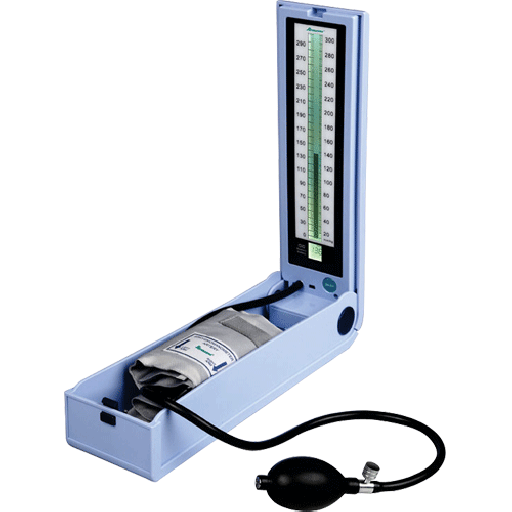
\includegraphics[width=0.45\textwidth,height=\textheight]{images/pngegg.png}
\end{center}

\subsection{Digital BP Monitor}\label{digital-bp-monitor}

\begin{quote}
A digital blood pressure (BP) monitor is an electronic device designed
to measure blood pressure and heart rate. It automates the process of
inflating the cuff, measuring the blood pressure, and displaying the
results, making it easier to use compared to traditional manual
sphygmomanometers.
\end{quote}

\begin{center}
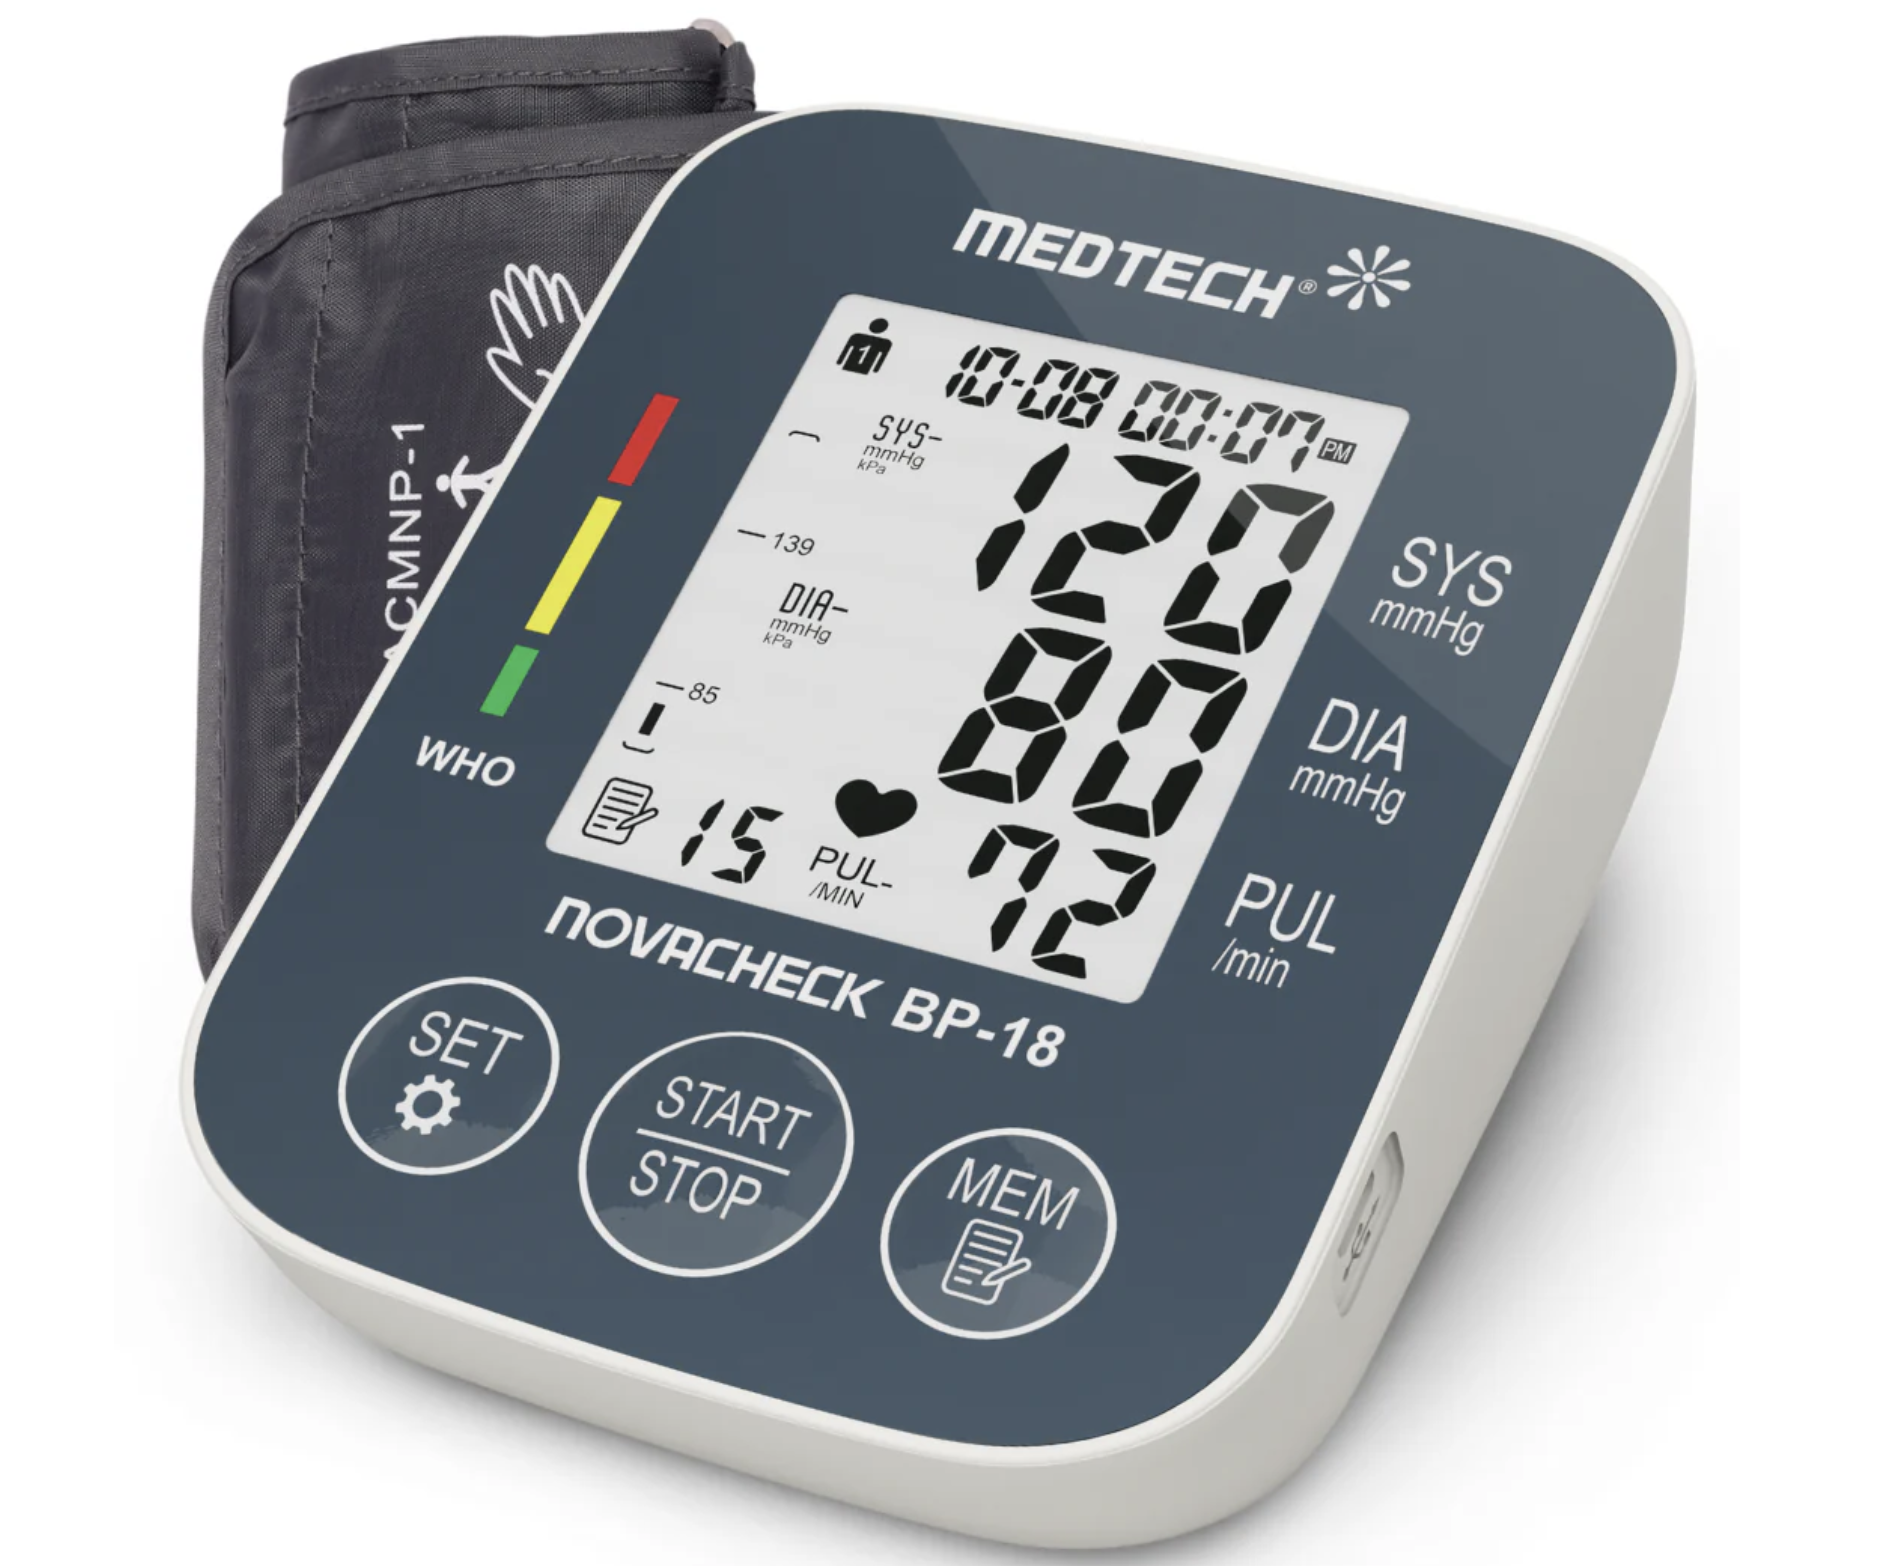
\includegraphics[width=4.5in,height=\textheight]{images/clipboard-3151283748.png}
\end{center}

\section{Procedure}\label{procedure}

\subsection{Sphygmomanometer}\label{sphygmomanometer-1}

\begin{itemize}
\item
  Subject is made to sit parallel to the mercury level of the monitor.
  The mercury knob is made opened.
\item
  Rough side of the cuff is placed on top of the left hand and is tied
  tightly on the brachial artery (point on left hand, where pulse is
  felt).
\item
  Stethoscope is placed on brachial artery just below the cuff's sensor
  to record Korotkoff's sounds (Heard when medical personnel listen for
  when they are taking blood pressure using a non invasive procedure).
\item
  The pressure is increased till 180mmHg using rubber bulb or inflator.
\end{itemize}

\subsubsection{Note}\label{note}

\begin{itemize}
\item
  Onset point of Korotkoff sound is the Systolic pressure
\item
  Dying of the Korotkoff sound is Diastolic pressure
\end{itemize}

\begin{quote}
and the readings are taken accordingly.
\end{quote}

\subsection{Digital Blood Pressure
Monitor}\label{digital-blood-pressure-monitor}

\begin{quote}
Digital sphygmomanometers are automated, providing blood pressure
reading without needing someone to operate the cuff or listen to the
blood flow.
\end{quote}

\section{Observation}\label{observation}

\setlength{\LTpost}{0mm}
\begin{longtable*}{lrrl}
\caption*{
{\large Observation table for Mechanical BP meter} \\ 
{\small Data taken from Mechanical BP meter}
} \\ 
\toprule
Student Name & BP Readings & Mean Arterial Pressure (MAP) & Analysis \\ 
\midrule\addlinespace[2.5pt]
Kulkarni sir & 120/80 & 93.33 & Normal \\ 
Monika & 110/70 & 83.33 & Normal \\ 
Kushaal & 130/90 & 103.33 & Pre-hypertension \\ 
Namyatha & 120/83 & 95.33 & Normal \\ 
Karthik & 125/85 & 98.33 & Pre-hypertension \\ 
Janane & 110/65 & 80.00 & Normal \\ 
Omar & 110/70 & 83.33 & Normal \\ 
Hasan & 100/70 & 80.00 & Normal \\ 
Saad & 120/85 & 96.66 & Normal \\ 
Manasa & 90/86 & 87.33 & Normal \\ 
Mayuri & 110/75 & 86.66 & Normal \\ 
Nidhi & 110/90 & 96.66 & Normal \\ 
Lakshita & 100/70 & 80.00 & Normal \\ 
\bottomrule
\end{longtable*}
\begin{minipage}{\linewidth}
Source: DTE Lab, 4th floor, Dept of Medical Electronics\\
\end{minipage}

\setlength{\LTpost}{0mm}
\begin{longtable*}{lrrl}
\caption*{
{\large Observation table for Digital BP meter} \\ 
{\small Data taken from Digital BP meter}
} \\ 
\toprule
Student Name & BP Readings & Mean Arterial Pressure (MAP) & Analysis \\ 
\midrule\addlinespace[2.5pt]
Kulkarni sir & 117/85 & 95.66 & Normal \\ 
Monika & 99/64 & 75.66 & Hypotension \\ 
Kushaal & 112/80 & 90.66 & Normal \\ 
Namyatha & 126/74 & 91.33 & Normal \\ 
Karthik & 119/80 & 93.00 & Normal \\ 
Janane & 112/70 & 84.00 & Normal \\ 
Omar & 117/67 & 83.66 & Normal \\ 
Hasan & 98/70 & 79.33 & Hypotension \\ 
Saad & 115/76 & 89.00 & Normal \\ 
Manasa & 82/69 & 73.33 & Hypotension \\ 
Mayuri & 115/76 & 89.00 & Normal \\ 
Nidhi & 100/80 & 86.66 & Normal \\ 
Lakshita & 85/73 & 77.00 & Hypotension \\ 
\bottomrule
\end{longtable*}
\begin{minipage}{\linewidth}
Source: DTE Lab, 4th floor, Dept of Medical Electronics\\
\end{minipage}

\section{Calculations}\label{calculations}

\[
MAP = \frac{1}{3} (SP - DP) + DP
\]

where \(MAP\) is Mean Arterial Pressure

\begin{description}
\item[Sphygmomanometer]
\[
\frac{1}{3} (120 - 80) + 80 = 93.33
\]
\item[Digital BP meter]
\[
\frac{1}{3} (117 - 85) + 85 = 95.66
\]
\end{description}

\section{Analysis}\label{analysis}

\begin{itemize}
\item
  We observe that there is a change in \texttt{MAP} with change in BP
  levels.
\item
  Generally, if there's a difference between systolic and diastolic
  pressure is \texttt{40\ mmHg}, the subject is considered to be normal.
\item
  If the difference between systolic and diastolic pressure ranges
  between \texttt{30\ -\ 50\ mmHg}, the subject is considered to be
  \texttt{normal} depending on the conditions.
\item
  If systolic and diastolic pressure difference is \(<30mmHg\), the
  subject has low BP which leads to hypotension.
\item
  If difference is \(>50mmHg\), the subject has high BP which leads to
  hypertension.
\end{itemize}

\section{Result}\label{result}

\begin{quote}
The working and analysis of mechanical and electronic BP meters are
analyzed.
\end{quote}

\bookmarksetup{startatroot}

\chapter{Electrocardiogram (ECG)
Measurement}\label{electrocardiogram-ecg-measurement}

\section{Aim}\label{aim-1}

\begin{quote}
Aquisition of ECG signal with the help of Power lab and Bio-pac systems.
\end{quote}

\section{Theory}\label{theory-1}

\begin{quote}
Electrocardiogram records from the body surface and registers the
differences in electrical potential generated by the heart. Signal
recorded is determined by action potentials generated by millions of
individual cells and their sequence of activation. A multitude of
factors (both cardiac and extracardiac) alter the final electrical
signal. For instance, the electrical forces generated by heart are
subsequently altered by the position of the heart within the body, the
nature of intervening tissue and the distance to the recording
electrode.
\end{quote}

\begin{itemize}
\item
  Lead 1 = RA, LA, RL
\item
  Lead 2 = RA, LL, RL
\item
  Lead 3 = LA, LL, RL
\end{itemize}

\begin{center}
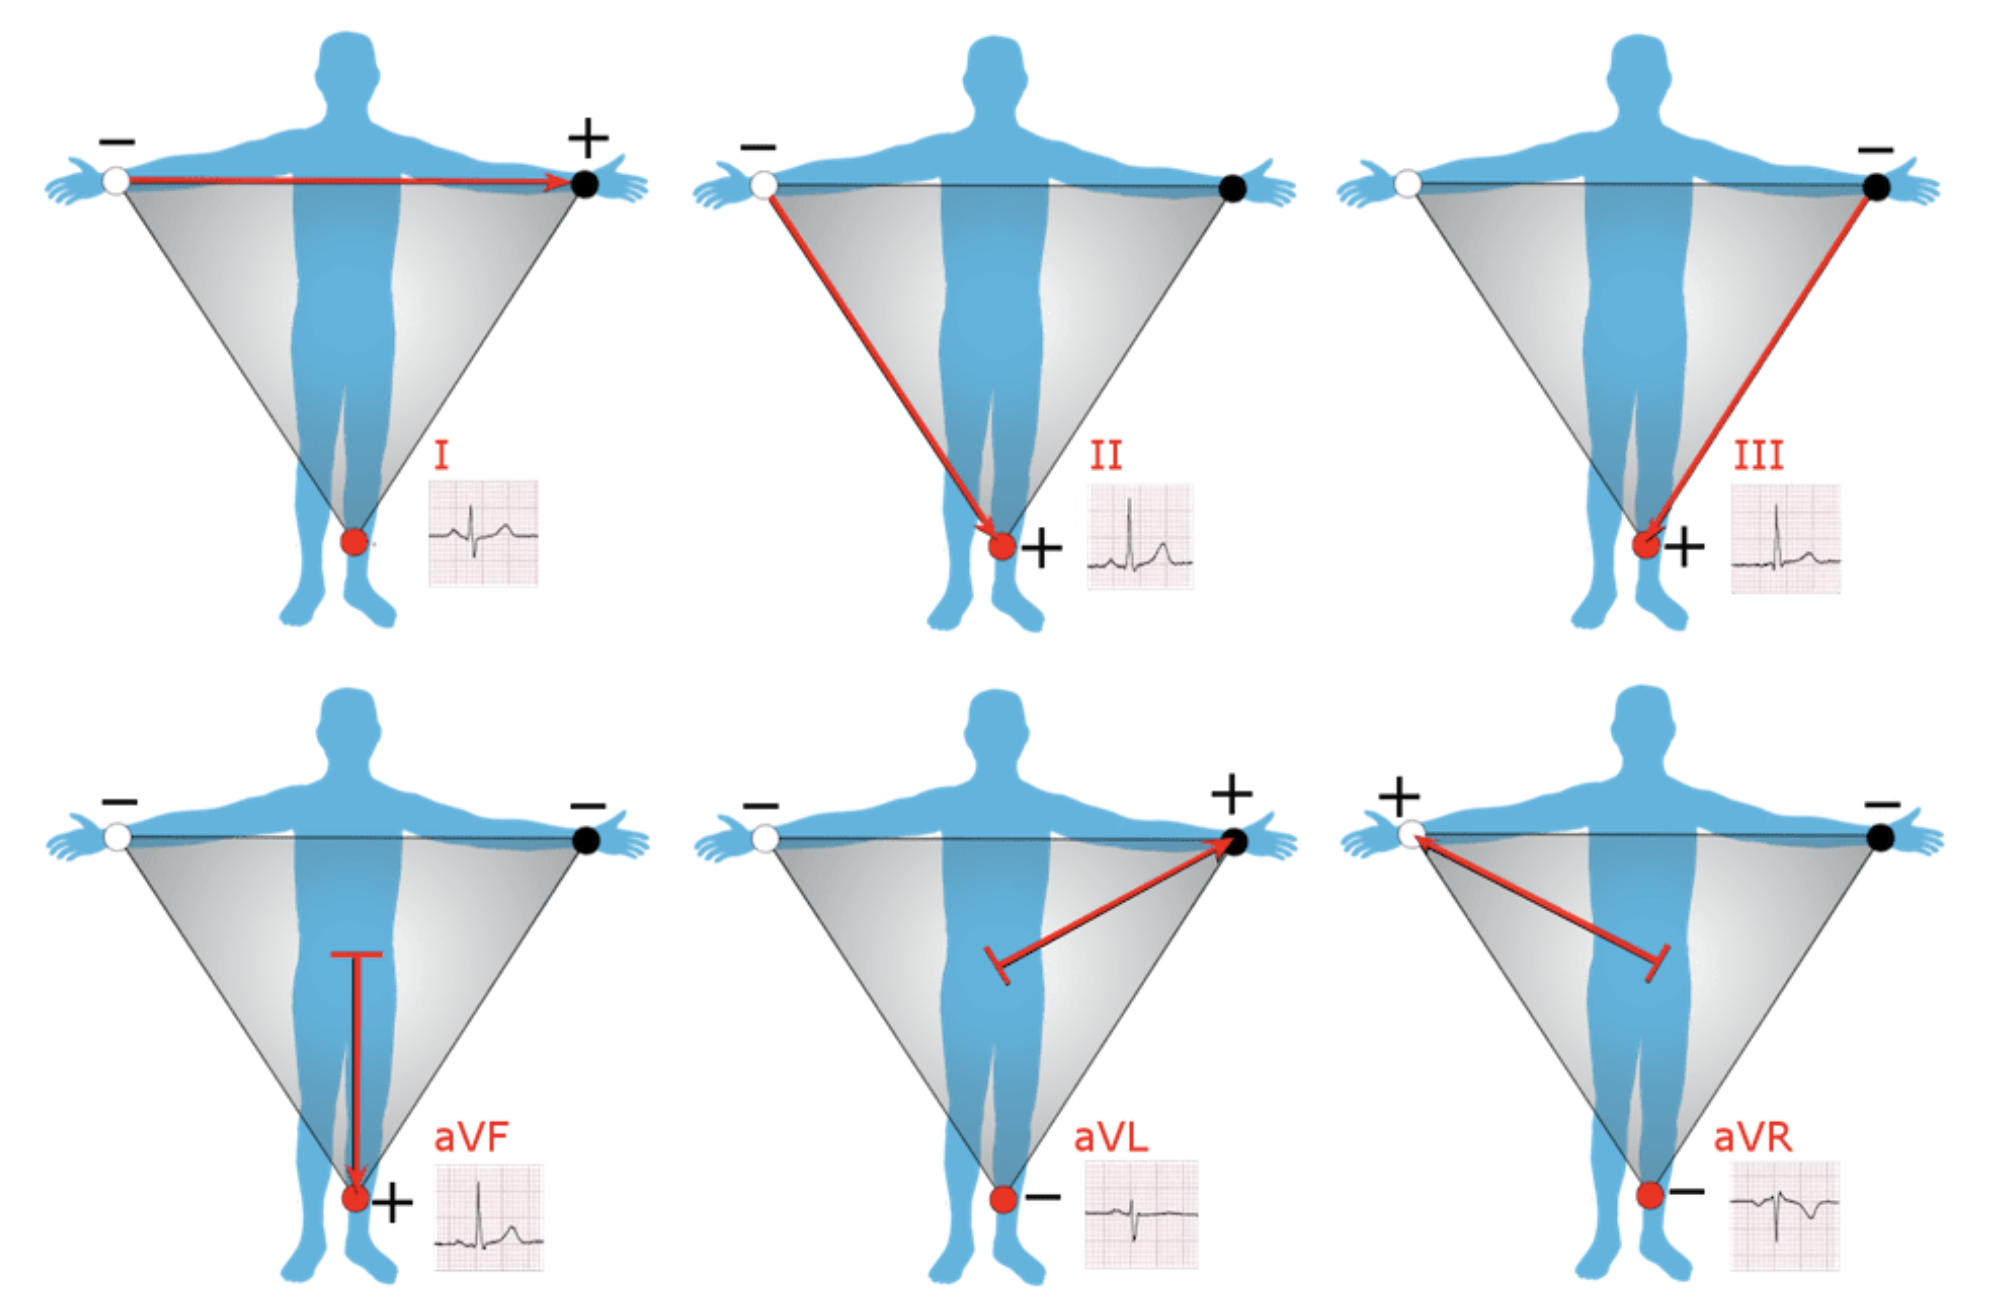
\includegraphics[width=5.82292in,height=\textheight]{images/clipboard-2797361598.png}
\end{center}

\begin{center}
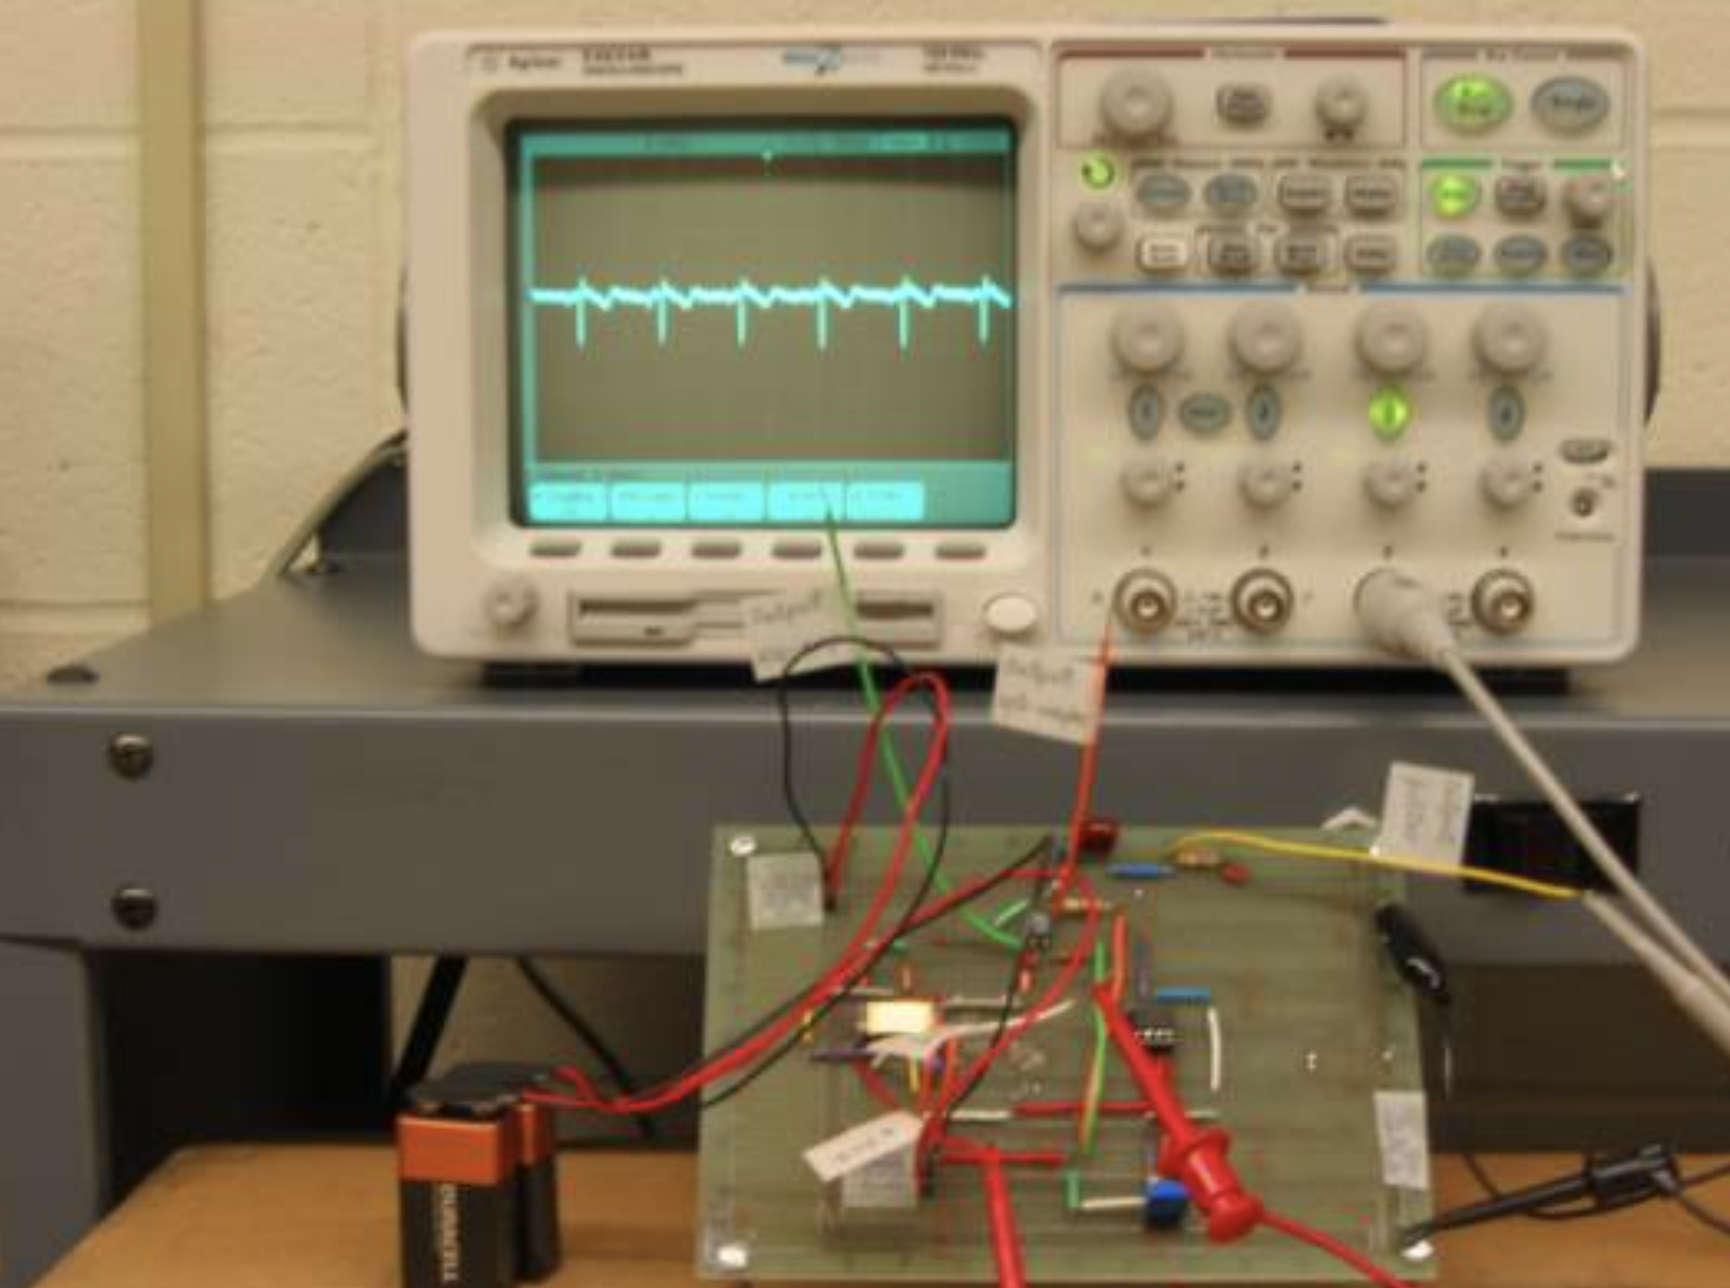
\includegraphics[width=0.48\textwidth,height=\textheight]{images/clipboard-91339677.png}
\end{center}

\begin{center}
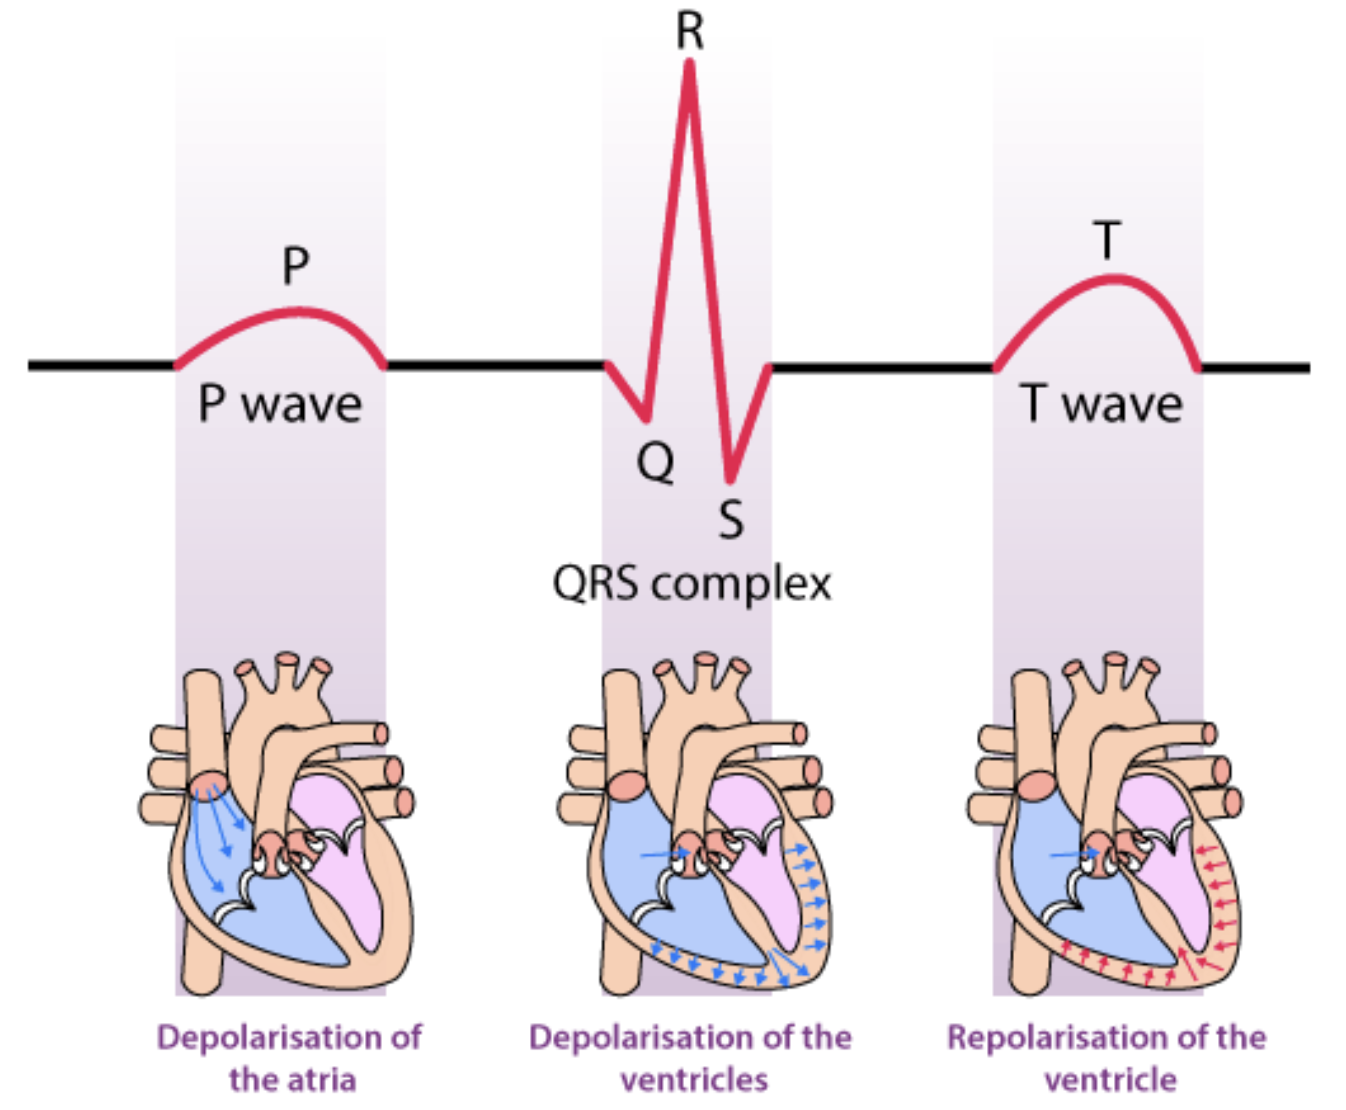
\includegraphics[width=0.51\textwidth,height=\textheight]{images/clipboard-1351516102.png}
\end{center}

\subsection{Bio-pac system}\label{bio-pac-system}

We aquire ECG signal using the Bio-pac system

\begin{center}
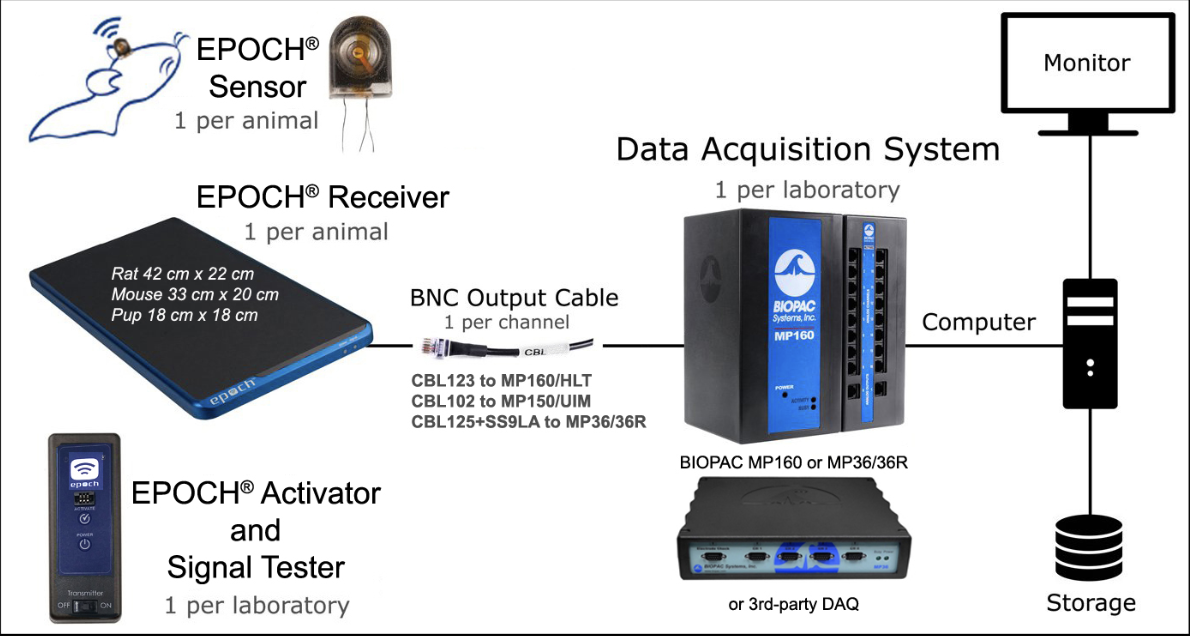
\includegraphics[width=0.74\textwidth,height=\textheight]{images/clipboard-1355974490.png}
\end{center}

\section{Procedure}\label{procedure-1}

\begin{enumerate}
\def\labelenumi{\arabic{enumi}.}
\tightlist
\item
  BIOPAC lessons are opened on the PC
\item
  Select \texttt{ECG1} and click OK.
\item
  Electrodes are placed on respective channel (CH:2) according to lead
  configurations. Transducer used is SS2L and subject should be at rest.
\item
  System is first calibrated and checked for proper contact of
  electrodes.
\item
  ECG setup is thus simulated, and the readings are recorded for each
  lead configuration
\item
  After recording the signals, BIOPAC lessons is clicked to save
  readings, which display the peak to peak voltage.
\item
  L1 + L3 = L2 is thus verified.
\end{enumerate}

\section{Observation}\label{observation-1}

\setlength{\LTpost}{0mm}
\begin{longtable*}{lrrrr}
\caption*{
{\large ECG Lead analysis} \\ 
{\small Peak-to-Peak Values, Frequencies, Time Intervals, and Beats per Minute (BPM) for ECG Leads}
} \\ 
\toprule
Lead Number & Peak to Peak & Frequency f (in Hz) & Time (in sec) = 1/f & Beats per Min = 60/T \\ 
\midrule\addlinespace[2.5pt]
Lead 1 & 0.47 & 1.27 & 0.78 & 76.92 \\ 
Lead 2 & 0.55 & 1.25 & 0.80 & 75.00 \\ 
Lead 3 & 0.08 & 1.26 & 0.79 & 75.94 \\ 
\bottomrule
\end{longtable*}
\begin{minipage}{\linewidth}
Source: DTE Lab, 4th floor, Dept of Medical Electronics\\
\end{minipage}

\section{Analysis}\label{analysis-1}

The Biopac software shows consistent heart rate readings across all
leads (75-77 bpm) indicating accurate and stable heart rate rhythm
detection.

ECG analysis if the subject is acquired and Lead1 + lead3 = Lead2 was
verified. Using frequency of the signal acquired, the bpm was also
found.

Lead 1 = 0.47

Lead 3 = 0.08

Lead 2 = 0.47 + 0.08 = 0.55

\(\frac{1}{f} = T = 0.78\) and \(\frac{60}{0.78} = 76.92\)

\section{Result}\label{result-1}

The ECG signal was aquired and L1 + L3 = L2 is verified.



\end{document}
